%kelompok 2
%Achmad Fatahillah(1154004)
%Ilga Anne Tri J.S(1154045)
%Maulyanda(1154008)
%Mefi Frinkazela Nikica(1154073)
%Simon Sorba Manangi(1154019)

\section{Variabel}
Pada sebagian besar bahasa pemrograman, nama suatu variabel
menjelaskan suatu nilai dengan tipe data tertentu 
dan menempati alamat memory yang pasti.
Variabel menyimpan data atau nilai yang dilakukan selama program dieksekusi,
Nilai variabel tersebut dapat diganti-ganti, namun tipe data selalu tetap.
Tidak demikian dengan python dimana tipe datanya dapat diubah-ubah
secara dinamis\cite{suparno2013komputasi}.

Variabel merupakan entitas yang memiliki nilai dan nilai tersebut berbeda satu dengan yang lain. Variabel mengalokasikan memori untuk menyimpan nilai.
Hal ini berarti ketika anda membuat variabel maka anda memesan beberapa ruang di memori. 
Variabel bisa digunakan untuk menyimpan bilangan bulat, desimal juga karakter.
Python sangat mementingkan indentasi, sehingga kita perlu melakukan indentasi secara konsisten. 
Indentitas tersebut dipermudah dengan menggunakan tombol Tab dan dimulai dari kolom pertama untuk setiap blok baru.\cite{santoso2009bahasa}


Variabel pada Python memiliki beberapa aturan seperti :
•	Case Sensitive : penggunaan huruf besar dan huruf kecil yang dibedakan.
•	Harus dimulai dengan underscore (_) atau huruf biasa, setelah itu dapat diikuti dengan huruf, angka atau underscore (_).
•	Tidak boleh mengandung karakter special seperti !,@,\#,\$ dan lainnya.
•	Hanya dapat menggunakan suatu variable setelah kita memberikan nilai ke dalamnya atau telah dilakukan assignment.
•	Setiap variable akan menyimpan referensi ke suatu objek dalam memory.\cite{santoso2009bahasa}


Variabel adalah sebuah nama yang selalu menunjukkan nilai tertentu. Dalam bahasa pemrograman Python, untuk membentuk sebuah variabel itu cukup hanya memberi nama pada nilai yang akan dibuat. Ini disebut dengan Assignment.
Contoh : 
>>>pesan="Halo, Semuanya"
Contoh di atas membuktikan bahwa itu adalah sebuah assignment, yang memberi kan sebuah nilai "Halo, Semuanya".\cite{Utami2004logika}

contoh lainnya:
\begin{equation}
>>> b = 2 # b bilangan bertipe integer
>>> print b
2
>>> b = b * 2.0 # Sekarang b bilangan bertipe float
>>> print b
4.0
\end{equation}
Tulisan b = 2 artinya kita memberi nilai pada variabel b dengan angka 2 yang bertipe integer
(bilangan bulat). Statemen berikutnya adalah melakukan operasi perkalian b ∗ 2.0 lalu hasilnya
disimpan pada variabel yang sama yaitu variabel b. Dengan demikian nilai b yang lama
akan diganti dengan nilai b yang baru, yaitu yang berasal dari operasi yang terakhir.
Sebagai Konsekuensi atau hasil dari operasi yang dirancang atau dibuat tersebut, 
sekarang variabel b memiliki tipe data float, 
suatu tipe yang berkaitan dengan bilangan pecahan atau desimal. 
Nilai variabel b menghasilkan nilai 4.0 atau empat\ref{pythonvariable}.
\begin{figure}[ht]
	\centerline{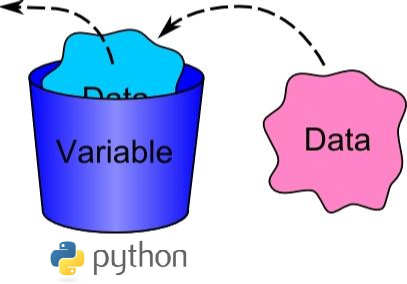
\includegraphics[width=0.25\textwidth]{figures/pythonvariable.png}
	\caption{gambar yang menggambarkan keadaan variabel pada python}
	\label{pythonvariable}
	\end{figure}

Tanda pagar (#) menyatakan awal dari suatu komentar. Komentar adalah bagian dari
script/program python yang tidak akan dieksekusi oleh interpreter. 


Python mementingkan indentasi, sehingga perlu indentasi yang konsisten. Indentasi dipermudah sesuai penggunaan
tombol Tab dan dimulai dari kolom pertama untu setiap blok baru. 

Bahasa pemrograman Python suatu fasilitas  shell di Linux, sehingga kita untuk mencoba penggunaan
Python secara leluasa. Lokasi instalan Python default pada distribusi Linux.

keunggulan Python adalah :
1. Python is powerful and fast = suatu kumpulan modul-modul yang sangat baik dan dapat menangani secara praktis setiap domain masalah
2. Python plays well with others = Python bisa berintegrasi dengan Component Object Model (COM) 
3. Python runs everywhere = versi Python berjalan di .NET, Java Virtual Machine dapat melihat bahwa sumber yang sama dapat berjalan tanpa perubahan berarti pada setiap sistem operasi tersebut.
4. Python is Open = Python dilisensi open source membuat Python digunakan dan disebarkan secara free,
5. Python is friendly and easy to learn = okumentasi yang lengkap merupakan salah satu fasilitas Python yang disenangi penggunanya. Apabila pembaca melakukan instalasi Python

Dalam menulis program, akan menggunakan code yang pernah kita  buat atau ditulis sebelumnya, pasti
kita gunakan kembali, dengan beberapa nilai berbeda.
 
Tentu saja tidak mungkin menuliskan kembali kode yang ingin dipanggil ulang tersebut.
Solusinya, supaya dapat dikelompokan kode-kode yang sering dipanggil ulang dalam suatu kelompok.

Selain itu dapat memecah masalah-masalah yang besar  menjadi masalah-masalah yang lebih kecil.
Dalam C atau bahasa pemrograman lain, biasanya digunakan istilah function.

Kemampuan python dalam mengelola tipe data sangat baik. Untuk mendeklarasikan suatu variabel dilakukan secara langsung tanpa menyebutkan tipe datanya, ini yang membedakan python dengan bahasa lain. Python akan menentukan tipe datanya secara otomatis. Python juga mendukung konversi dan perhitungan antar tipe data dengan ketelitian yang tinggi. Python membagi tipe data ke dalam 2 jenis bilangan (semua tipe yang berhubungan dengan angka murni) dan string. Untuk tipe data dalam rumpun bilangan termasuk didalamnya adalah integer, long, float, oktal, hexadimal dan bilangan kompleks. Hal-hal yang harus diperhatikan :
•	Untuk bilangan oktal dan hexa masing-masing diawali dengan 0 dan 0x
•	Untuk bilangan panjang diakhiri menggunakan karakter l atau L
•	Untuk bilangan float, gunakan e atau E pada eksponensial
•	Untuk bilangan kompleks dibagi ke menjadi bagian real dan imajiner, dan diakhiri dengan j atau J Operator untuk tipe dalam rumpun bilangan.\cite{utamipemrograman}

\subsection{Membuat Variabel}
Variabel atau peubah memiliki pengertian sembarang symbol yang dapat dimuati oleh sembarang himpunan bilangan. Dalam pengertian komputasi sebuah nama yang digunakan untuk menyimpan nilai dengan kapasitas tertentu dan alamat tertentu dalam memori komputer. Variabel merupakan pendaftaran tipe data bagi variabel, konstanta dan parameter yang digunakan sebuah program agar mempunyai alamat penyimpanan dan kapasitas data dalam memori komputer. Dalam membuat variabel hindari spasi dan menggunakan karakter khusus, selain itu juga nama dalam kata cadangan Python (seperti input, eval, if, elif, for, def, dan lain-lain) tidak dapat menjadi variabel.\cite{irfani2016bahan}

Nama variabel atau disebut juga dengan identifier dalam bahasa pemrograman Python juga dapat berupa kumpulan dari huru (letter) maupun angka (digit) yang dengan cara membedakan huruf kecil dan juga huruf besar, Karakter pertama pada identifier harus berupa huruf dan juga perlu diketahui bahwa penggunaan karakter garis bwah itu juga dapat digunakan.
